\documentclass[11pt,a4paper]{article}

\usepackage[margin=2.5cm]{geometry}
\usepackage[T1]{fontenc}
\usepackage[utf8]{inputenc}
\usepackage{lmodern}
\usepackage{amsmath,amssymb}
\usepackage{graphicx}
\usepackage{booktabs}
\usepackage{multirow}
\usepackage{caption}
\usepackage{tikz}
\usetikzlibrary{positioning,arrows.meta}
\usepackage[hidelinks]{hyperref}

\graphicspath{{figures/}}
\captionsetup{font=small,labelfont=bf}

\title{Context-Aware Stress Detection from Wearable Heart-Rate Variability:\\
Zero-Shot Chronos-2 versus Classical Baselines}
\author{Nikola Jankovikj (259076)\\[2pt]\small Ambient Intelligence}
\date{November 2026}

\begin{document}
\maketitle

\begin{abstract}
Wearables record physiology all day, which makes them an obvious sensing layer for ambient intelligence. Heart-rate variability (HRV) drops under psychological stress, but it moves just as much with physical activity, posture and sleep, so a context-aware system has to read HRV \emph{given} what the user is doing.

We test whether Chronos-2, a pretrained time-series foundation model, can supply this context-awareness \emph{zero-shot}. Chronos-2 forecasts a person's HRV (RMSSD) from its recent history, optionally together with activity covariates, and the deviation from the forecast serves as the anomaly score. We compare it with classical baselines on two public datasets: a laboratory stress protocol (WESAD, 15 subjects) and 24-hour free-living recordings (MMASH, 20 subjects).

In the lab, every univariate method separates stress from the person's resting baseline with a median AUROC of about $0.96$, and Chronos-2 is not meaningfully better than the context mean (95\% CI of the difference $-0.070$ to $+0.010$). Covariates make Chronos-2 \emph{worse} ($-0.235$ AUROC) because during stress they leave the range seen in the context. In free-living data they make no difference either way. All models detect an unexplained 30\% RMSSD drop only weakly (AUROC $0.61$ to $0.66$), and activity causes few false alarms in the first place.

The foundation model works as an anomaly scorer, but it is no better than the simple ones. Context only helps when the context the model sees already contains the variation it has to explain.
\end{abstract}

% ---------------------------------------------------------------------------
\section{Introduction}

Ambient intelligence (AmI) describes environments that are sensitive and responsive to the people in them~\cite{cook2009ami}. Wearable devices extend this sensing to the body: a chest strap or wrist device records heartbeats, movement and skin responses continuously, without the user doing anything. An AmI system for well-being could use these streams to notice when a person is under stress and react, for example by suggesting a break or adapting the environment.

Heart-rate variability is the most widely used physiological stress marker. Its short-term component, RMSSD, reflects parasympathetic activity, which is withdrawn under acute stress, so RMSSD typically falls~\cite{taskforce1996hrv,shaffer2017hrv,kim2018stress}. The trouble is that RMSSD also falls during exercise and standing, and rises during sleep. A system that flagged every low-RMSSD period would mostly flag people walking around. Reading a measurement \emph{in context} is the kind of problem an AmI system is supposed to handle.

Time-series foundation models are one way to try. Chronos-2~\cite{ansari2025chronos2} is pretrained on a large corpus of time series and forecasts new series without any training. Unlike its predecessor~\cite{ansari2024chronos}, it accepts \emph{covariates}, i.e.\ other series that may explain the target. If it can forecast a person's RMSSD from their recent history and current activity, then whatever part of RMSSD it \emph{cannot} forecast is a candidate stress signal. This needs no labelled stress data and no model fitted per user, and real deployments rarely have either.

\paragraph{Goal and thesis.} We evaluate this idea against simple classical baselines and test two claims:
\begin{enumerate}
  \item \textbf{Detection (lab, WESAD).} Forecast residuals from zero-shot Chronos-2 detect stress-induced HRV changes better than classical baselines, and covariates improve detection.
  \item \textbf{Context-awareness (free living, MMASH).} With activity, posture and sleep covariates, Chronos-2 avoids false alarms during physical activity while staying sensitive to RMSSD changes that the covariates do not explain.
\end{enumerate}

\paragraph{Contributions.} We build a reproducible pipeline that turns raw ECG or RR data into a 1\,Hz RMSSD signal aligned with activity covariates, and a residual-based anomaly score that is the same for every model. We define two evaluation protocols with comparisons fixed in advance, one of them a paired injection design for free-living data that has no labels. With these we compare Chronos-2, with and without covariates, against static and dynamic classical baselines, and run diagnostics that show \emph{why} covariates help or hurt. Neither claim holds up, and the reasons are useful for anyone building context-aware AmI systems.

% ---------------------------------------------------------------------------
\section{Background}

\paragraph{HRV and stress.} RMSSD is the root mean square of successive differences between heartbeat (RR) intervals:
\begin{equation}
  \mathrm{RMSSD} = \sqrt{\frac{1}{N-1}\sum_{i=1}^{N-1}\left(RR_{i+1}-RR_i\right)^2}.
\end{equation}
It is stable on windows as short as one minute, whereas frequency-domain measures need about five~\cite{shaffer2017hrv}, so it suits near-continuous monitoring. How it responds to stress varies between individuals~\cite{kim2018stress}.

\paragraph{Wearable stress detection.} Most work on WESAD~\cite{schmidt2018wesad} trains supervised classifiers on hand-crafted features from several sensors, which requires labelled stress episodes from comparable users. We take the unsupervised view instead: learn what is \emph{normal} for a person and flag deviations from it.

\paragraph{Forecasting-based anomaly detection.} A forecaster predicts the next values of a signal, and large standardised residuals are flagged as anomalies~\cite{hundman2018telemanom}. How good such a detector is depends on how well the forecaster models normal behaviour and its uncertainty.

\paragraph{Chronos and Chronos-2.} Chronos~\cite{ansari2024chronos} tokenises time series and applies a language-model architecture to forecast univariate series zero-shot. Chronos-2~\cite{ansari2025chronos2} extends this to multivariate inputs: the target is processed jointly with \emph{past-only} covariates (known only up to the present) and \emph{known-future} covariates (also given for the forecast horizon). It outputs a set of forecast quantiles. We use the 28M-parameter \texttt{chronos-2-small} model on CPU.

% ---------------------------------------------------------------------------
\section{Data}

Table~\ref{tab:data} summarises both datasets.

\textbf{WESAD}~\cite{schmidt2018wesad} is a laboratory study with 15 subjects (the authors removed S1 and S12 because of sensor faults). A chest RespiBAN records ECG, three-axis acceleration, electrodermal activity (EDA), respiration and skin temperature at 700\,Hz. The labelled conditions are a seated baseline of about 20\,min, psychosocial stress from the Trier Social Stress Test (TSST: public speech and mental arithmetic~\cite{kirschbaum1993tsst}), and amusement and meditation, with unlabelled transitions in between. Seven subjects did stress first and eight did amusement first. Stress begins 17 to 44\,min after the end of the resting reference used in Phase~1.

\textbf{MMASH}~\cite{rossi2020mmash,goldberger2000physionet} contains about 24\,h of free-living recordings from 22 healthy adults. RR intervals come from a Polar H7 chest strap, and an ActiGraph wGT3X-BT records acceleration, steps and inclinometer posture. The dataset also includes in-bed periods (\texttt{sleep.csv}), a self-reported activity log (exercise, eating, caffeine, smoking, alcohol), a Daily Stress Inventory score, and saliva cortisol at bedtime and on waking. Before any scoring we excluded two users, one with 18.6\% RR artifacts and one with no sleep record, which leaves 20 subjects.

\begin{table}[t]
  \centering\small
  \caption{Datasets as used in this project.}
  \label{tab:data}
  \begin{tabular}{p{2.7cm}p{6cm}p{6cm}}
    \toprule
    & WESAD (Phase 1) & MMASH (Phase 2) \\
    \midrule
    Setting & Laboratory protocol & Free living, $\sim$24\,h \\
    Subjects used & 15 & 20 (of 22) \\
    Heart signal & Chest ECG, 700\,Hz & Polar H7 RR intervals \\
    Context signals & HR, ACC magnitude, EDA, respiration rate, skin temp. & Movement, steps, posture, in-bed, activity log \\
    Ground truth & Stress (TSST) vs baseline labels & None (semi-synthetic positives) \\
    RR artifact rate & 0.0 to 3.0\% per subject & 0.0 to 6.4\% per subject \\
    \bottomrule
  \end{tabular}
\end{table}

% ---------------------------------------------------------------------------
\section{Data transformation}

We convert both datasets into the same representation: a 1\,Hz table with the RMSSD target and time-aligned covariates. Figure~\ref{fig:pipeline} shows the pipeline.

\begin{figure}[t]
  \centering
  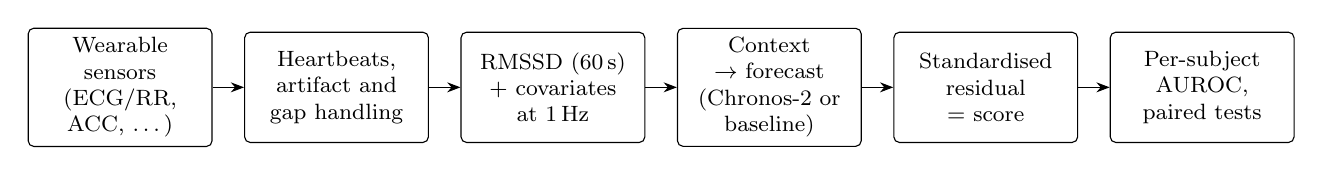
\begin{tikzpicture}[node distance=4mm, >=Stealth,
      box/.style={draw, rounded corners=2pt, align=center, text width=21mm,
                  minimum height=14mm, font=\footnotesize}]
    \node[box] (a) {Wearable\\ sensors\\ (ECG/RR, ACC, \dots)};
    \node[box, right=of a] (b) {Heartbeats,\\ artifact and\\ gap handling};
    \node[box, right=of b] (c) {RMSSD (60\,s)\\ + covariates\\ at 1\,Hz};
    \node[box, right=of c] (d) {Context\\ $\rightarrow$ forecast\\ (Chronos-2 or\\ baseline)};
    \node[box, right=of d] (e) {Standardised\\ residual\\ $=$ score};
    \node[box, right=of e] (f) {Per-subject\\ AUROC,\\ paired tests};
    \foreach \src/\dst in {a/b, b/c, c/d, d/e, e/f} \draw[->] (\src) -- (\dst);
  \end{tikzpicture}
  \caption{Processing and evaluation pipeline, shared by both phases.}
  \label{fig:pipeline}
\end{figure}

\paragraph{Heartbeats.} For WESAD, we clean the 700\,Hz chest ECG and detect R-peaks with NeuroKit2~\cite{makowski2021neurokit2}; RR intervals are the differences between peaks. MMASH provides RR intervals directly but needed two fixes. Two users have their second recording day encoded as $-29$, which we map back to day 2. And every recording has 2{,}200 to 2{,}700 gaps of 5 to 10\,s per day where beats were not transmitted.

\paragraph{Artifact handling.} An RR interval is rejected if it lies outside 300 to 2000\,ms, or if it deviates by more than 20\% from the median of its five neighbours. Rejected intervals are marked as missing rather than deleted, and a missing marker is inserted after every recording gap. Successive differences are therefore only ever taken between two \emph{adjacent} valid beats. Deleting the intervals would instead join beats that were not neighbours and inflate RMSSD; in an early version of the pipeline this pushed one subject's stress RMSSD from 64 to 72\,ms.

\paragraph{RMSSD at 1\,Hz.} For every second $t$, RMSSD is computed over the beats in the trailing 60\,s. In MMASH a value is kept only if the window contains at least 20 valid successive differences, which holds for 82 to 100\% of seconds per subject. Consecutive values overlap by 59\,s, so the series is smooth, and this matters for the evaluation (Section~\ref{sec:protocol}).

\paragraph{Covariates.} All covariates are resampled to the same 1\,Hz grid. For WESAD they are heart rate, acceleration magnitude, EDA, respiration rate (0.1 to 0.5\,Hz band-pass followed by peak detection) and skin temperature, each mean-pooled to 1\,Hz. For MMASH they are the 60\,s trailing means of acceleration vector magnitude and of steps per minute, the fraction of the trailing minute spent lying or standing, an in-bed flag, and activity-log flags for exercise, eating and stimulants. We checked the activity codes against the dataset documentation.

In MMASH we deliberately leave heart rate out. It is computed from the same heartbeats and responds to stress itself, so a model could use it to forecast away the signal it is meant to detect (Section~\ref{sec:results1}).

% ---------------------------------------------------------------------------
\section{Method}

\subsection{Anomaly score}
Each model receives a \emph{context}, i.e.\ the history before a time $s$, and outputs a point forecast $\hat y_t$ and a scale $\hat\sigma_t$ for the following steps. A scored window $W$ of 30\,s gets the score
\begin{equation}
  S(W) = \frac{1}{|W|}\sum_{t\in W}\frac{\lvert y_t-\hat y_t\rvert}{\hat\sigma_t}.
  \label{eq:score}
\end{equation}
The score is two-sided because in five WESAD subjects RMSSD \emph{rises} under stress. Every model uses the same score, so the models differ only in how well they predict normal behaviour and its uncertainty.

\subsection{How Chronos-2 is used}
We use Chronos-2 strictly zero-shot, with no fine-tuning and no fitting to any subject. For each scoring position, the context (RMSSD and, in the covariate variant, the covariate history) is passed to \texttt{predict\_df}. The covariate values over the forecast horizon go in as known-future inputs (\texttt{future\_df}), since a wearable measures activity at the same time as the heart. Chronos-2 returns the quantiles $q_{0.1}, q_{0.5}, q_{0.9}$. We take $\hat y=q_{0.5}$ and convert the 80\% interval to a standard deviation, $\hat\sigma=(q_{0.9}-q_{0.1})/2.563$ (the Gaussian ratio), so its scores are in the same units as the baselines'. In MMASH, about 270 positions per subject are forecast in one batched call.

\subsection{Comparison models}
All models see exactly the same context and the same covariates.
\begin{itemize}
  \item \textbf{SMA (context mean):} $\hat y$ and $\hat\sigma$ are the mean and standard deviation of the context. This is the simplest possible reference.
  \item \textbf{ARIMA / ARIMAX} (Phase 1): a SARIMAX$(2,0,2)$ fitted per subject on the context. The ARIMAX variant forecasts with the window's covariates, and $\hat\sigma$ is the forecast standard error.
  \item \textbf{OLS + covariates} (Phase 2): a linear regression of RMSSD on the covariates over the context, i.e.\ the static, context-aware counterpart of SMA. Covariates that are constant in the context are dropped.
  \item \textbf{Persistence $\pm$ covariates} (Phase 2): the classical \emph{dynamic} baseline. The last RMSSD value is carried forward, optionally corrected by $\beta^\top(x_t-x_{\text{last}})$, where $\beta$ is fitted on $k$-step RMSSD changes against $k$-step covariate changes within the context. $\hat\sigma$ is the empirical $k$-step error. (Refitting ARIMAX for each of about 5{,}400 windows was not feasible on CPU.)
\end{itemize}
Each family has a variant without covariates (context-blind) and one with covariates (context-aware), so the effect of context can be separated from the effect of the model.

\subsection{Evaluation protocols}\label{sec:protocol}

\paragraph{Phase 1: personal baseline (WESAD).} The context is the last 300\,s of the first two-thirds of the subject's resting baseline. Negatives are held-out baseline windows that start 60\,s after the context, so they share no heartbeat with it, and positives are all stress windows. The question being asked is: \emph{given five minutes of this person at rest, is this window anomalous?} We first tried a rolling context, and it fails for a structural reason. Stress begins 17 to 44\,min after the baseline, so by the time a stress window is scored the rolling context already contains stress, and every method scored AUROC $\approx 0.47$. As a control, we also compare stress with amusement and meditation windows, which are just as far in time from the context but are not stressful.

\paragraph{Phase 2: paired injection (MMASH).} MMASH has no stress labels, so we measure sensitivity semi-synthetically. Every 300\,s, a model receives the preceding 30\,min and forecasts 90\,s ahead. Only the last 30\,s are scored, so their 60\,s RMSSD contains no heartbeat from the context. Each window is scored twice, once as recorded (negative) and once with its RMSSD multiplied by $(1-d)$, $d=30\%$ (positive). Because the scored values contain only post-context beats, this injection is exactly what a 30\% reduction of every heartbeat difference after time $s$ would produce: an abrupt RMSSD drop that the covariates do not explain. Both versions share the same context and forecast, so the drop is the \emph{only} thing that differs between them. The primary metric is the per-subject AUROC of injected versus real windows. Activity false alarms are measured as the AUROC of real \emph{active} windows ($\geq$60 steps/min or logged exercise) against real sedentary awake windows, where 0.5 means activity is not flagged.

An earlier version scored the window directly after the context and had no dynamic baseline. It gave Chronos-2 a spurious advantage ($0.96$ vs $0.65$), because the first scored RMSSD values were mostly built from beats the model had already seen. We added the 60\,s guard and the persistence family to remove this artefact.

\subsection{Statistics}
The subject is the unit of analysis, since windows within a subject are not independent. We compare models with the paired Wilcoxon signed-rank test~\cite{wilcoxon1945} on per-subject AUROC, with Holm correction~\cite{holm1979} within each pre-specified family of comparisons. We report the mean paired difference with a 95\% bootstrap confidence interval over subjects, and the matched-pairs rank-biserial correlation $r$.

A difference counts as practically meaningful only if it exceeds $\pm0.05$ AUROC. If the CI lies inside this margin we call the methods \emph{equivalent}; if only one bound lies inside it, the corresponding method is \emph{not meaningfully better}. A non-significant test on its own is never read as ``no difference''.

% ---------------------------------------------------------------------------
\section{Results}

\subsection{Phase 1: laboratory stress (WESAD)}\label{sec:results1}

\begin{table}[t]
  \centering\small
  \caption{Phase 1, median over 15 subjects. Primary: stress vs held-out baseline. Control: stress vs amusement and meditation.}
  \label{tab:p1}
  \begin{tabular}{llccc}
    \toprule
    & Model & AUROC (primary) [IQR] & AUPRC & AUROC (control) \\
    \midrule
    \multirow{3}{*}{Univariate} & SMA & 0.955 [0.859, 1.000] & 0.981 & 0.785 \\
    & ARIMA & 0.968 [0.883, 1.000] & 0.987 & 0.704 \\
    & Chronos-2 & 0.959 [0.878, 1.000] & 0.983 & 0.688 \\
    \midrule
    \multirow{2}{*}{+ covariates} & ARIMAX & 1.000 [0.947, 1.000] & 1.000 & 0.968 \\
    & Chronos-2 & 0.660 [0.357, 0.895] & 0.811 & 0.560 \\
    \bottomrule
  \end{tabular}
\end{table}

\begin{figure}[t]
  \centering
  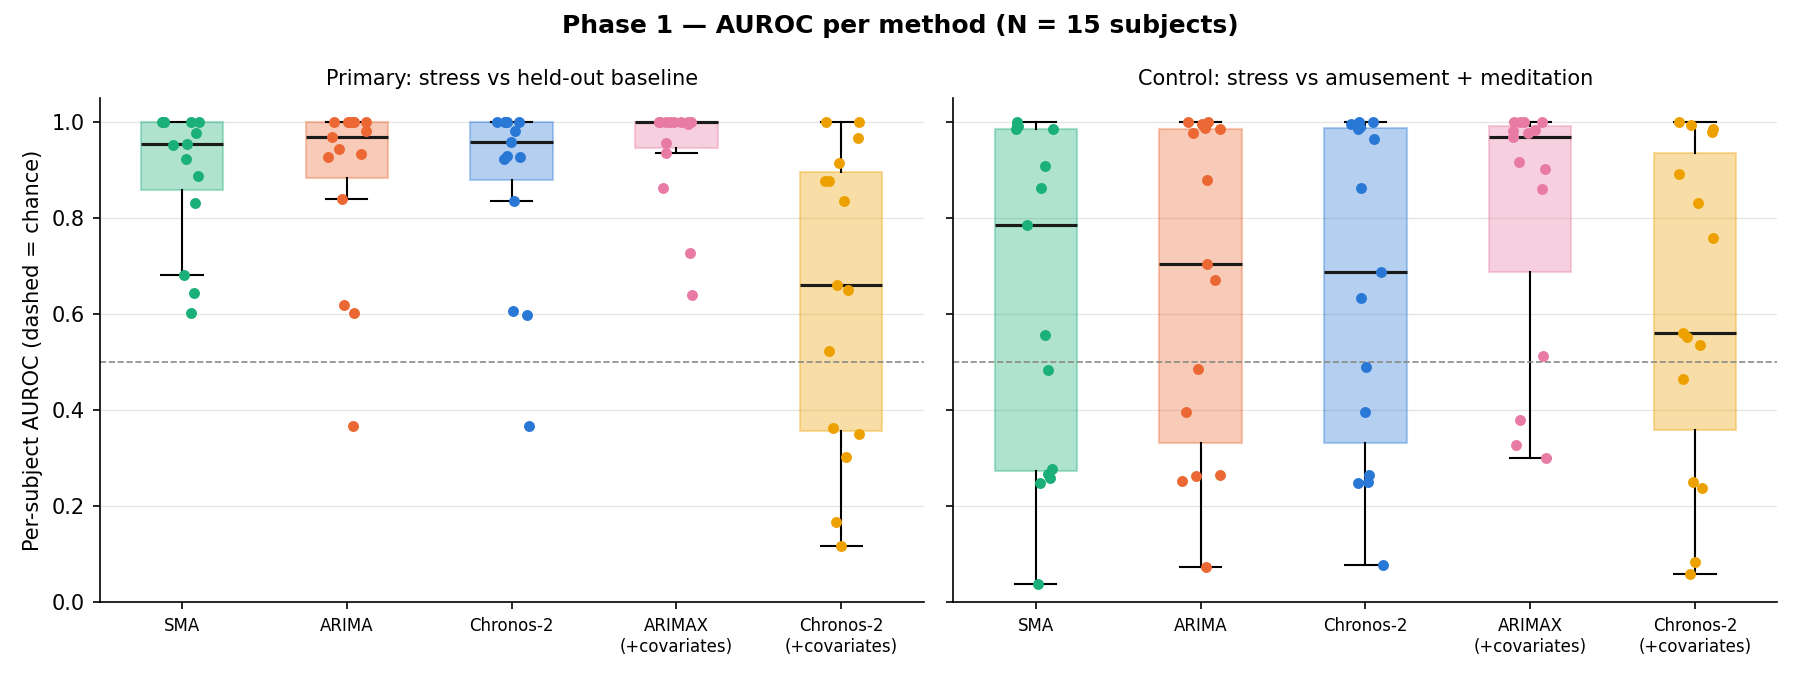
\includegraphics[width=\textwidth]{fig1_auroc_summary.png}
  \caption{Phase 1 per-subject AUROC. Left: stress vs held-out baseline. Right: stress vs amusement and meditation (control). Dashed line: chance.}
  \label{fig:p1}
\end{figure}

\paragraph{Univariate comparison.} Against a five-minute resting reference, every univariate method detects stress well (Table~\ref{tab:p1}, Figure~\ref{fig:p1}). In the ten subjects whose RMSSD falls under stress, all three reach a median AUROC of 1.000. The five subjects whose RMSSD rises hold every method back by the same amount (medians 0.61 to 0.68). Chronos-2 is not meaningfully better than SMA (mean difference $-0.022$, 95\% CI $[-0.070, +0.010]$, $p_\text{Holm}=0.70$). It is marginally worse than ARIMA on every subject where the two differ ($-0.004$, CI $[-0.007, -0.001]$, $p_\text{Holm}=0.031$), but that difference sits far inside the equivalence margin.

With a fixed reference, each univariate model is essentially estimating the person's resting level and spread, and five minutes of data are enough for any method to pin those down. The control task shows where the score runs out. Against amusement and meditation the medians drop to 0.69 to 0.79, because what the score detects is \emph{deviation from rest}, and stress just happens to be the largest deviation.

\begin{table}[t]
  \centering\small
  \caption{Phase 1 covariates during stress relative to the 5-min rest context (median over subjects), and the AUROC of the covariate models when the observed RMSSD is replaced by the context mean (``flat RMSSD'').}
  \label{tab:ood}
  \begin{tabular}{lccccc}
    \toprule
    & EDA & Skin temp. & Resp.\ rate & HR & ACC \\
    \midrule
    Stress values outside the context range & 100\% & 100\% & 46\% & 32\% & 13\% \\
    Mean shift (context SDs) & 42.3 & 6.7 & 1.4 & 3.0 & 4.6 \\
    \midrule
    \multicolumn{6}{l}{Flat-RMSSD AUROC: ARIMAX + covariates 1.000; Chronos-2 + covariates 0.065} \\
    \bottomrule
  \end{tabular}
\end{table}

\paragraph{Covariates.} Adding the five covariates makes Chronos-2 clearly worse: $-0.235$ AUROC, CI $[-0.363, -0.130]$, $p_\text{Holm}<0.001$, with every non-tied subject worse. Table~\ref{tab:ood} shows why. During the TSST every covariate moves far outside anything seen in the seated rest context; EDA, for example, is 42 context standard deviations away. When Chronos-2 gets covariate values it has never seen, it widens its forecast interval instead of shifting the forecast, and that shrinks the score in Eq.~\eqref{eq:score} in precisely the stress windows. With RMSSD held flat, the covariates alone rank stress windows \emph{below} baseline windows (AUROC 0.065).

ARIMAX with covariates reaches a perfect median of 1.000, but this is not HRV anomaly detection, since it stays at 1.000 when RMSSD is held flat. A linear model fitted on almost-constant covariates and extrapolated to stress-level EDA and HR produces forecasts that have nothing to do with RMSSD, so the model ends up working as a multimodal stress detector by accident. WESAD therefore cannot test the covariate claim: the rest context has no non-stress covariate variation to learn from, and every covariate responds either to the stressor or to the act of speaking.

\begin{figure}[t]
  \centering
  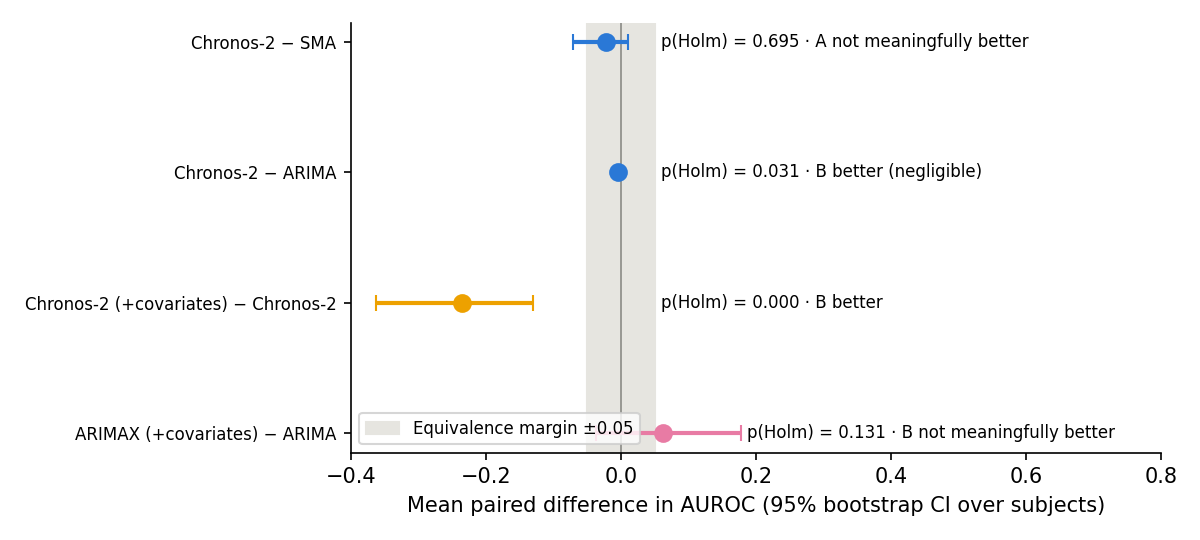
\includegraphics[width=0.85\textwidth]{fig4_paired_differences.png}
  \caption{Phase 1 planned comparisons: mean paired AUROC difference with 95\% bootstrap CI. Shaded: $\pm0.05$ equivalence margin.}
  \label{fig:p1forest}
\end{figure}

\subsection{Phase 2: free living (MMASH)}

\begin{table}[t]
  \centering\small
  \caption{Phase 2, median over 20 subjects. Injection: AUROC of a 30\% unexplained RMSSD drop vs real windows (overall and within states). Activity alarms: AUROC of real active vs sedentary windows (0.5 = activity not flagged).}
  \label{tab:p2}
  \begin{tabular}{llccccc}
    \toprule
    Family & Model & Injection & Sedentary & Active & Sleep & Activity alarms \\
    \midrule
    \multirow{2}{*}{Static} & SMA & 0.660 & 0.656 & 0.631 & 0.677 & 0.546 \\
    & OLS + cov & 0.645 & 0.645 & 0.588 & 0.689 & 0.533 \\
    \midrule
    \multirow{2}{*}{Dynamic} & Persistence & 0.621 & 0.608 & 0.603 & 0.694 & 0.505 \\
    & Persistence + cov & 0.613 & 0.607 & 0.582 & 0.677 & 0.525 \\
    \midrule
    \multirow{2}{*}{Foundation} & Chronos-2 & 0.645 & 0.636 & 0.585 & 0.751 & 0.528 \\
    & Chronos-2 + cov & 0.654 & 0.632 & 0.611 & 0.719 & 0.511 \\
    \bottomrule
  \end{tabular}
\end{table}

\begin{figure}[t]
  \centering
  \begin{minipage}{0.56\textwidth}
    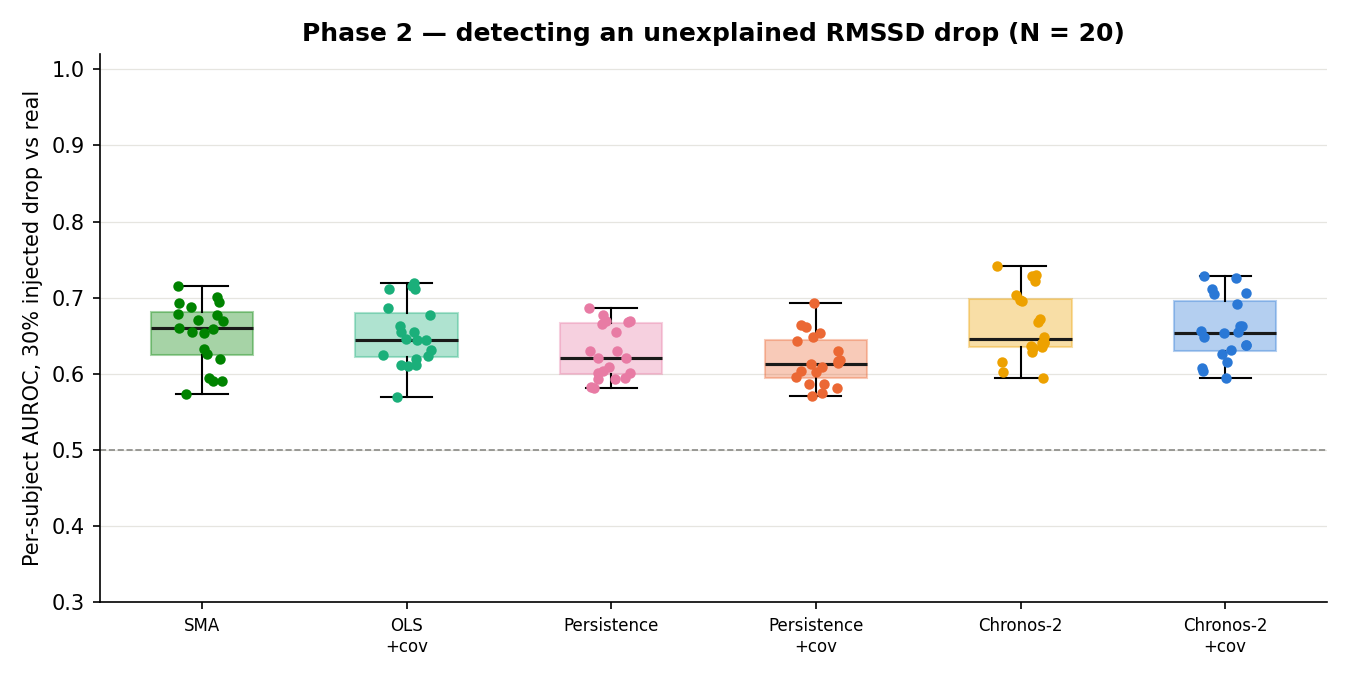
\includegraphics[width=\textwidth]{fig6_phase2_injection_auroc.png}
  \end{minipage}\hfill
  \begin{minipage}{0.42\textwidth}
    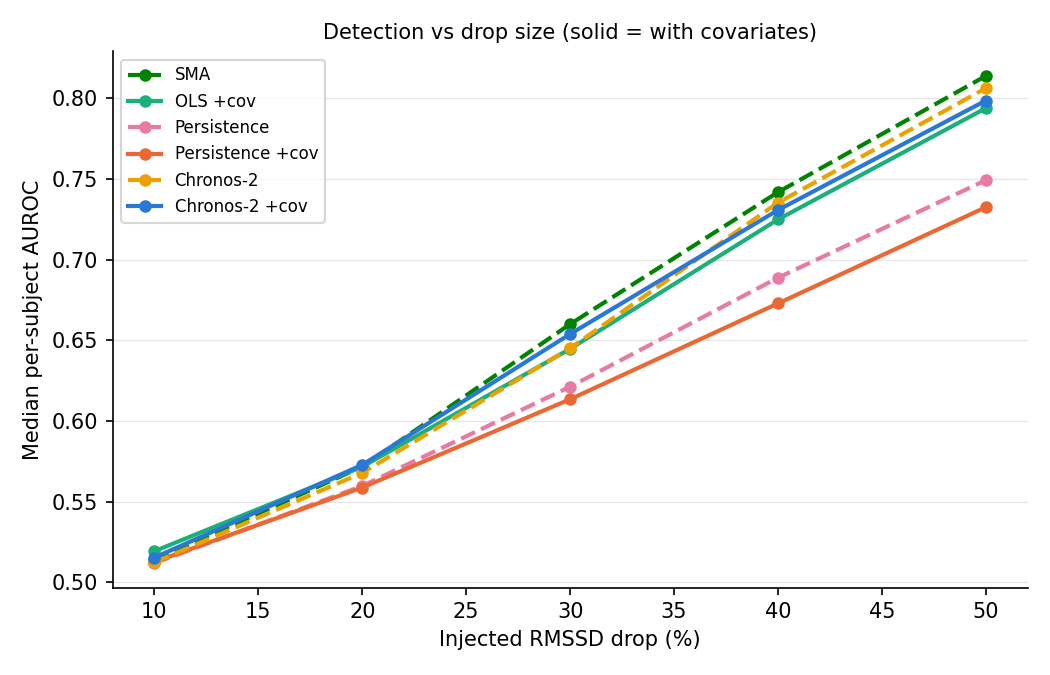
\includegraphics[width=\textwidth]{fig7_phase2_depth_sweep.png}
  \end{minipage}
  \caption{Phase 2. Left: per-subject AUROC for a 30\% injected drop. Right: median AUROC as a function of drop size (solid lines: with covariates).}
  \label{fig:p2}
\end{figure}

\paragraph{Sensitivity.} Every model struggles to detect an unexplained RMSSD drop 60 to 90\,s after it starts (Table~\ref{tab:p2}, Figure~\ref{fig:p2}). A 30\% drop gives median AUROCs of 0.61 to 0.66. A 50\% drop, which is larger than the average TSST response in WESAD (about 47\%), gives 0.73 to 0.81. The highest median belongs to the context mean (SMA).

\paragraph{Planned comparisons (Figure~\ref{fig:p2forest}).} Covariates do not help Chronos-2 (difference $-0.006$, CI $[-0.013, +0.002]$, $p_\text{Holm}=0.14$), and the two variants are equivalent. Chronos-2 with covariates beats persistence with covariates on every subject ($+0.040$, CI $[+0.032, +0.047]$, $p_\text{Holm}<0.001$), but the whole CI lies inside the equivalence margin, so the advantage is negligible. Against SMA, in an unplanned and purely descriptive comparison, the difference is $+0.006$, CI $[-0.009, +0.020]$.

\paragraph{Activity false alarms.} Activity barely raises scores even \emph{without} covariates (median AUROC 0.505 to 0.546), and adding covariates does not change this significantly in any family ($p_\text{Holm}\geq0.115$). With a rolling 30\,min context, all models already adapt to the person's current level and spread, which leaves few false alarms for context to remove. Unlike in the lab, covariates do not hurt Chronos-2 here, because only 2 to 3\% of movement and posture values in the forecast span fall outside the range of the 30\,min context. This fits the out-of-range explanation from Phase 1.

\paragraph{Exploratory.} We correlated each subject's mean sedentary score with their daily stress score and with their wake-minus-bedtime cortisol change. One of the 12 correlations is nominally significant ($\rho=0.46$, $p=0.046$, $n=19$), which is about what chance would give, and none survives correction.

\begin{figure}[t]
  \centering
  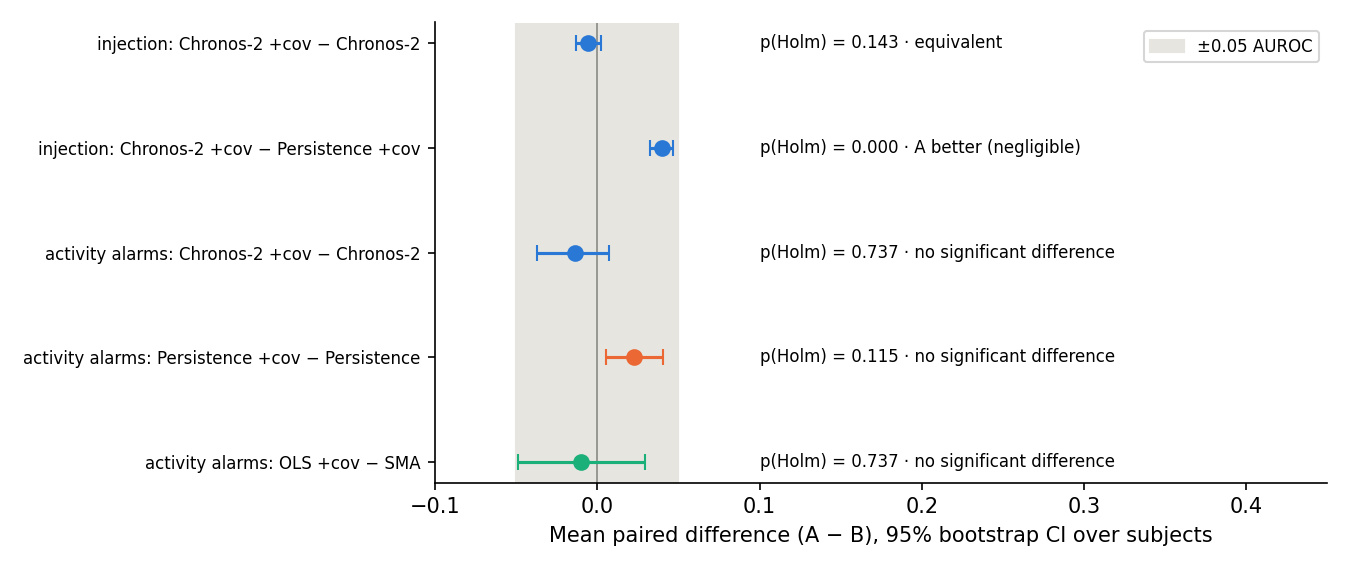
\includegraphics[width=0.85\textwidth]{fig9_phase2_comparisons.png}
  \caption{Phase 2 planned comparisons with 95\% bootstrap CIs. Injection: higher is better. Activity alarms: lower means fewer alarms during activity.}
  \label{fig:p2forest}
\end{figure}

% ---------------------------------------------------------------------------
\section{Discussion}

\paragraph{Comparison with the baselines.} In both settings the zero-shot foundation model matches the classical baselines but does not beat them. In the lab it is equivalent in practice to the context mean and to ARIMA. In free living it beats naive persistence by a consistent but small margin and does not beat the context mean. One result is encouraging for an AmI deployment: a single pretrained model that was never fitted to anyone performs as well as models fitted per subject. It adds no detection power, though, and costs far more to compute.

\paragraph{When does context help?} The covariate results, negative in the lab and neutral in free living, have the same cause. A forecaster can only use context to \emph{explain} a change in RMSSD if its history shows how RMSSD responds to that context. In the lab the history is a stretch of seated rest, and stress moves every sensor far outside it, so Chronos-2 reacts with uncertainty and ARIMAX with extrapolation. In free living the 30\,min history contains ordinary activity transitions, so the covariates stay within the range the model has seen. But then the history on its own already captures most of the activity effect, and the covariates have little left to explain.

For context-aware AmI systems this means that sensing the context is not enough. The model also has to see that context vary under \emph{normal} conditions, and the context signals must not respond to the target state themselves (HR and EDA do respond to stress).

\paragraph{Methodological lessons.} Several evaluation choices that looked reasonable gave misleading results during the project and had to be corrected:
\begin{itemize}
  \item A rolling context hides sustained stress (AUROC $\approx0.47$).
  \item Scoring windows whose smoothed RMSSD overlaps the context inflated Chronos-2 to 0.96 in free living.
  \item An early implementation passed covariates only as history, so the lab result that ``covariates do not matter'' was true by construction.
  \item Deleting artifact beats inflated RMSSD.
\end{itemize}
We caught each one by asking what information a model could legitimately have, and by adding controls: the time-distance control, holding RMSSD flat, and the covariate-range check. Wearable data with overlapping windows and wired-in context signals is especially prone to leaks like these.

\section{Limitations and future work}

The samples are small (15 and 20 subjects). The confidence intervals bound the effects, but subgroups such as the subjects whose RMSSD rises under stress remain uncertain.

The positives in Phase 2 are synthetic. The injected drops are abrupt and come without the posture or heart-rate changes that go along with real stress. Free-living data with momentary stress reports would allow a direct test.

We evaluated only \texttt{chronos-2-small}, and the context length, window length and guard were fixed in advance rather than tuned. The 120M model, longer contexts, and contexts that deliberately include varied activity are the natural next steps.

Finally, subjects may have changed posture during the TSST, which affects RMSSD independently of stress, and acceleration magnitude cannot capture posture.

\section{Conclusion}

We asked whether a time-series foundation model can give a wearable stress detector context-awareness without per-user training. In the lab, zero-shot Chronos-2 detects stress against a personal baseline (median AUROC $0.96$), but no better than the context mean or ARIMA, and covariates hurt it because the stressor pushes them outside anything the context contains. In 24\,h free-living data the covariates are neutral, every model detects unexplained HRV drops only weakly, and physical activity produces few false alarms for context to remove.

Neither project claim is supported. The pipeline, protocols and diagnostics can be reused, and the main finding applies to ambient intelligence more broadly: context helps a model only when the model has seen that context vary under normal conditions.

\bibliographystyle{plain}
\bibliography{references}

\end{document}
